\documentclass{article}
\usepackage{graphicx,psfrag,epsfig,epsf,latexsym,hhline,amsmath,amssymb,multirow}
\usepackage[usenames,dvipsnames]{pstricks}
\usepackage{pst-plot}
\usepackage{pstricks-add}
%\IEEEoverridecommandlockouts
\usepackage{color}
\usepackage{stmaryrd}

\interdisplaylinepenalty=2500
\usepackage{graphicx}
\usepackage{amsthm}
\usepackage{footnote}

\usepackage{blindtext}
\usepackage{etoolbox}

\usepackage{tikz}
\usepackage{pgfplots}
\usepgflibrary{shapes}
\usetikzlibrary{arrows,shapes,chains,matrix,positioning,scopes,patterns	}
\pgfplotsset{compat=newest}
\pgfplotsset{plot coordinates/math parser=false}

\begin{document}

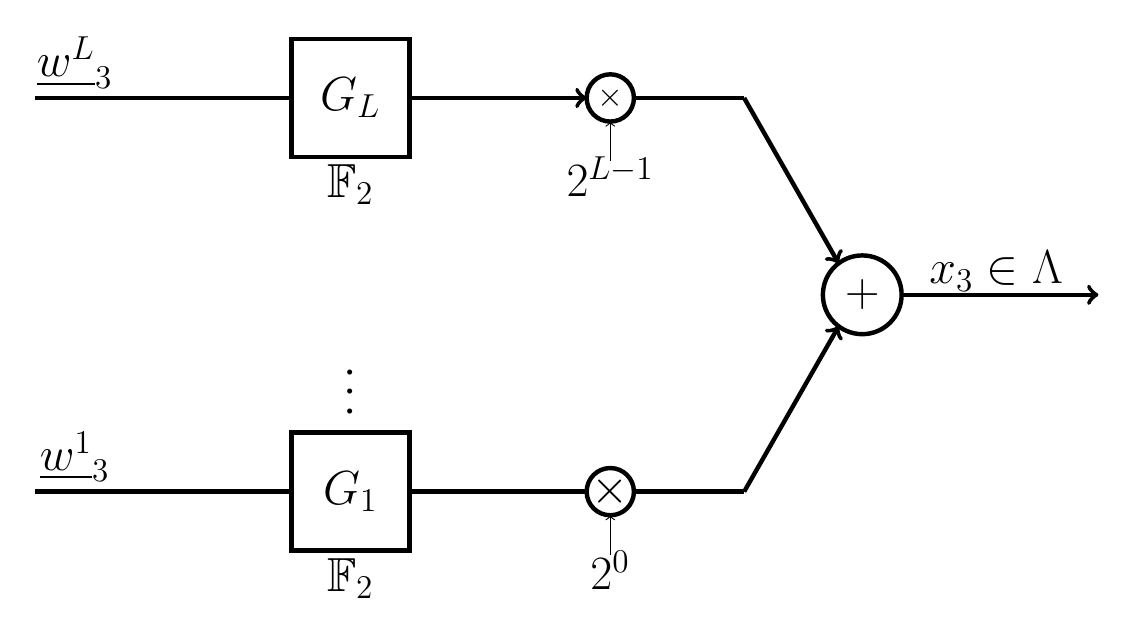
\begin{tikzpicture}[scale=1]

%Uncoded level
%\draw [ultra thick](-3,2.5) -- (6.2,2.5);
%\node [above, font=\large] at (-2.5,2.5){$2^{L}\mathbb{Z}^{N}$} ;

%Oblique lines to Plus block
\draw[->][ultra thick](6,1) -- (7.2,-1.1);
\draw[->][ultra thick](6,-4) -- (7.2,-1.9);
%\draw[->] [ultra thick](6.2,2.5) -- (7.2,-1.1);

%Code blocks
\draw [ultra thick] (0.25,0.25) rectangle (1.75,1.75); \node [font=\LARGE] at (1,1){$G_{L}$} ;
\draw [ultra thick] (0.25,-4.75) rectangle (1.75,-3.25); \node [font=\LARGE] at (1,-4){$G_{1}$} ;

%Line extensions to Code blocks
\draw[ultra thick] (-3,1) -- (0.25,1);  \node [above, font=\LARGE] at (-2.5,1){$\underline{w^L}_{3}$} ;
\draw [ultra thick](-3,-4) -- (0.25,-4); \node [above, font=\LARGE] at (-2.5,-4){$\underline{w^1}_{3}$} ;
 \draw[ultra thick][->] (1.75,1) -- (4,1);   \draw [ultra thick](1.75,-4) -- (4,-4);
\node [font=\LARGE] at (1,-0.1){$\mathbb{F}_{2}$} ;
\node [font=\LARGE] at (1,-5.1){$\mathbb{F}_{2}$} ;

%Multiplication blocks and lines to them
\draw [ultra thick](4.3,1) circle (0.3); \node [font=\large] at (4.3,1){$\times$} ;
\draw [ultra thick](4.3,-4) circle (0.3);  \node [font=\LARGE] at (4.3,-4){$\times$} ;
\draw [ultra thick](4.6,1) -- (6,1); \draw [ultra thick](4.6,-4) -- (6,-4);

\draw [<-] (4.3,0.7) -- (4.3,0.2);\node [font=\LARGE] at (4.3,0){$2^{L-1}$} ;
\draw [<-] (4.3,-4.3) -- (4.3,-4.8); \node [font=\LARGE] at (4.3,-5){$2^{0}$} ;

%cdots
\node [font=\LARGE] at (1,-2.75){$\cdot$} ;
\node [font=\LARGE] at (1,-2.5){$\cdot$} ;
\node [font=\LARGE] at (1,-3){$\cdot$} ;

%Plus block and extensions
\draw [ultra thick](7.5,-1.5) circle (0.5);
\node [font=\LARGE] at (7.5,-1.5){+} ;

\draw [ultra thick][->] (8,-1.5) -- (10.5,-1.5);
 \node [font=\LARGE] at (9.2,-1.2){$x_3 \in \Lambda$} ;

 \end{tikzpicture}

\end{document} 